\documentclass{report}
\usepackage[fontsize=13pt]{scrextend}

\usepackage{my_lab}

\begin{document}

\MiptLabTitle{4.2.4}{ИНТЕРФЕРОМЕТР МАЙКЕЛЬСОНА}

\begin{document}
\textbf{Цель работы}: Изучение двухлучевой интерференции, определение дли-
ны волны, проверка эффекта Доплера.

\textbf{В работе используется}: интерферометр Майкельсона с подвижным зер-
калом, лазер, ффотоумножитель, частотомер, линзы.

\section*{Установка}
\begin{figure}[H]
	\centering
	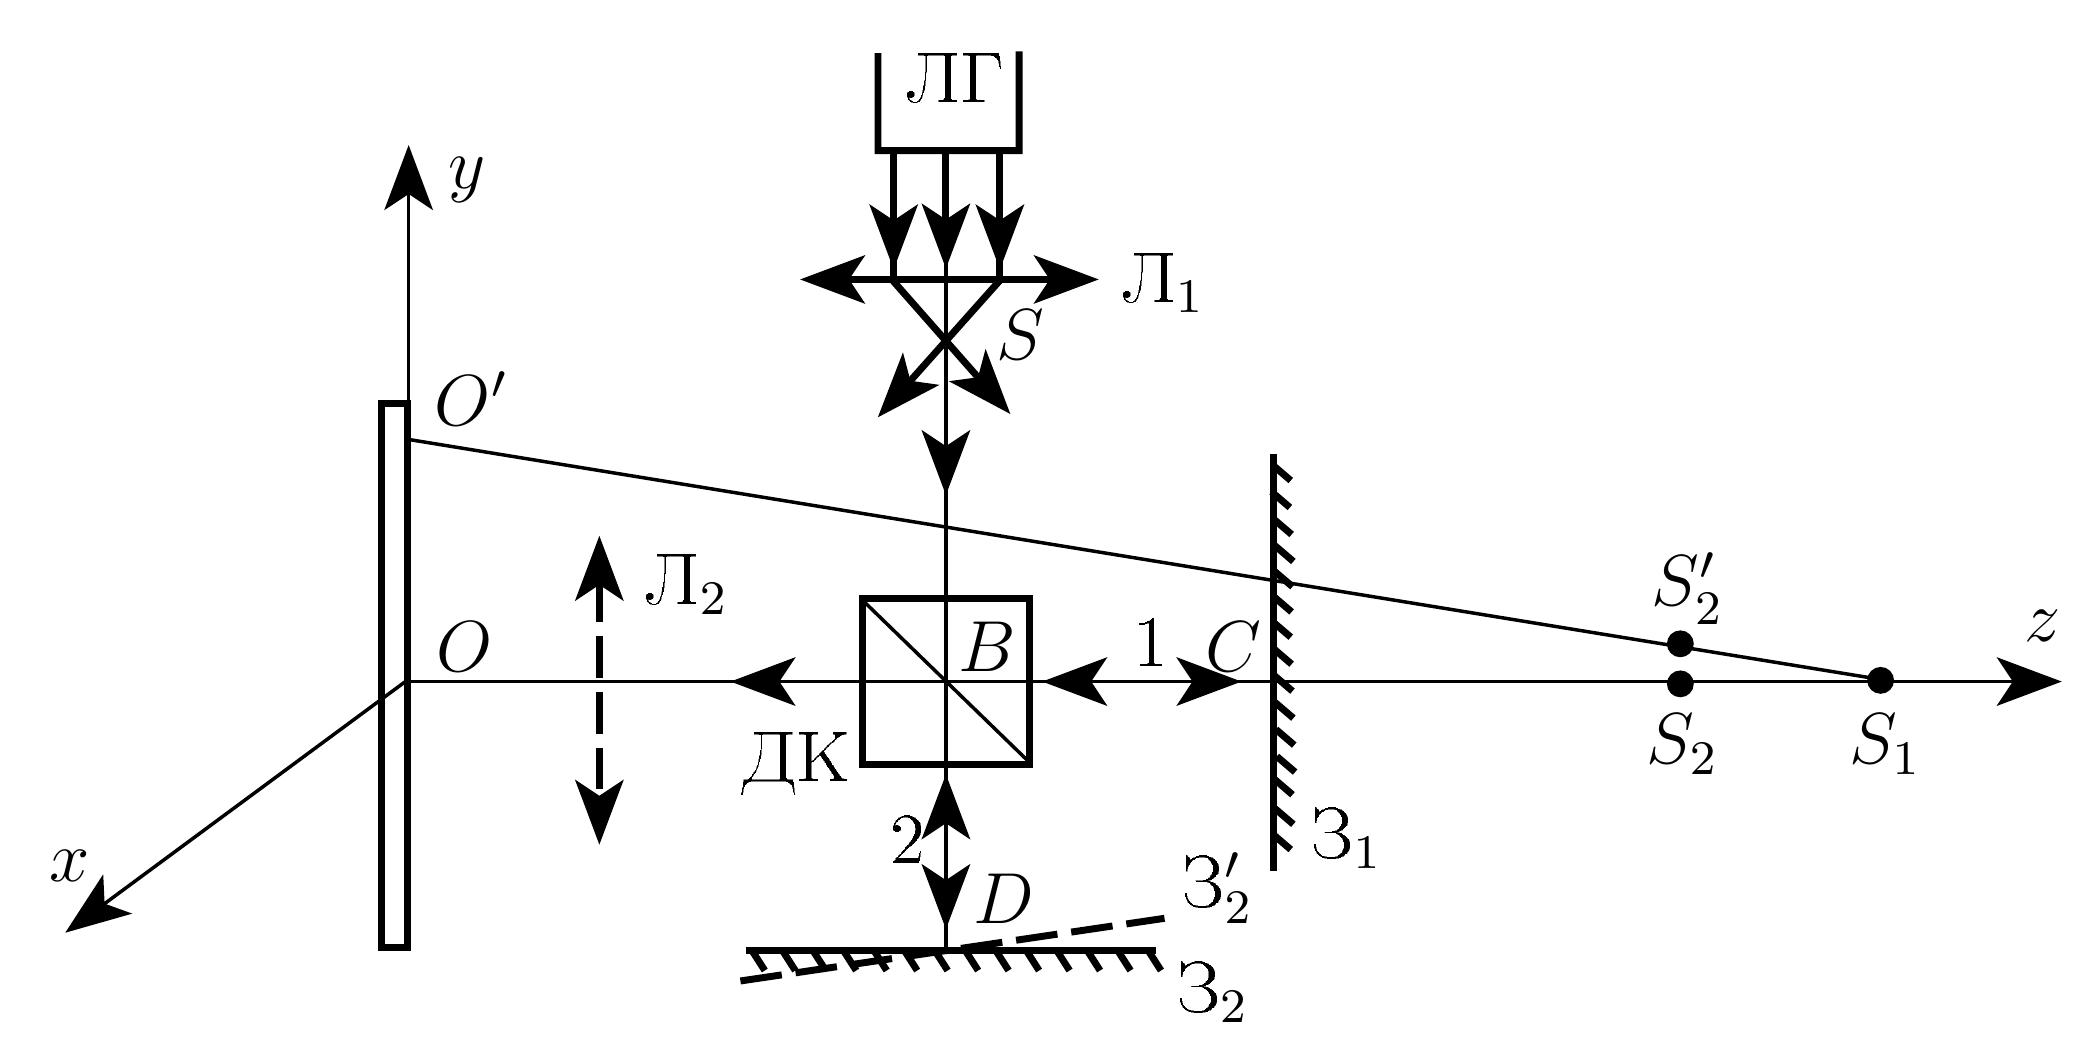
\includegraphics[width=0.9\linewidth]{figures/schema1.png}
	\caption{Схема интерферометра}
\end{figure}
\begin{description}
	\item[ДК] - делительный кубик.
	\item[ЛГ] - гелий-неоновый лазер ЛГН-203.
	\item[$L_1, L_2$] - линзы.
	\item[$\text{З}_1, \text{З}_2$] - зеркала. \\
	      З1 закреплено, З2 можно поворачивать.
	\item[Э] - экран в точке О, для наблюдения интерференции. \\
\end{description}

\begin{figure}[H]
	\centering
	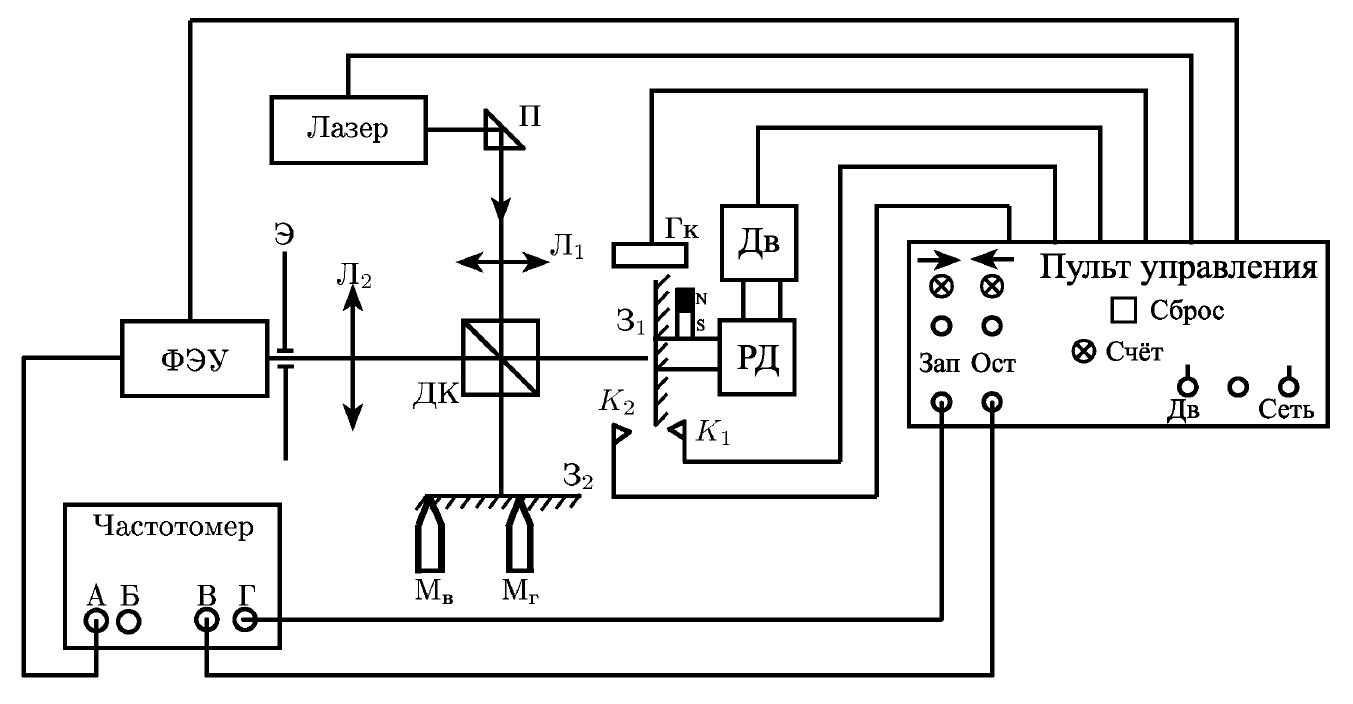
\includegraphics[width=0.9\linewidth]{figures/schema2.png}
	\caption{Схема экспериментальной установки}
\end{figure}
\begin{description}
	\item[ДВ] - двигатель, который меняет положение З1.
	\item[РД] - редуктор, может менять вкорость ДВ.
	\item[ФЭУ] - фотоэлектронный умножитель ФЭУ-68, для регистрации изменения интенсивности света.
\end{description}

Изменение положения З1 приводит к периодическому изменению интенсивности на Э. \\
Эти изменения фиксируются и подсчитываются частотомером.

\section*{Теоретическая часть}

\section*{Ход работы}

\section{Юстировка системы}
Получим интерференционную картину (и.к.) на экране. \\
Для этого расположим элементы установки как на схеме. \\
Э, З1 и Л фиксированы. Можно передвигать линзы и поворачивать З2. \\
Удачи...

\section{Исследование интерференционной картины}
\begin{enumerate}
	\item Разместим центр и.к. в центре экрана.
	\item Запишем радиусы пяти-шести первых тёмных колец. \\
	      Убедимся в справедливости формулы (2.69): \\
	      \begin{equation}
		      r_n \approx \sqrt{2nL(L - a) / m_0}
	      \end{equation}
	      $\D L = a = S_2 S_2^{'} = 2(BC - BD)$ - разница хода \\
	      $L = S_1 O$\\
	      $m_0 = \frac{\D L}{\lambda} \approx 1.2 \cdot 10^5$ - порядок интерференции \\

	      \begin{table}[H]
		      \centering
		      \begin{tabular}{|l|l|l|l|l|l|}
			      \hline
			      $n$        & 1   & 2   & 3   & 4   & 5   \\
			      \hline
			      $r_n, \mm$ & 0.5 & 1.0 & 1.5 & 1.7 & 2.2 \\
			      \hline
		      \end{tabular}
	      \end{table}

	      \begin{figure}[H]
		      \centering
		      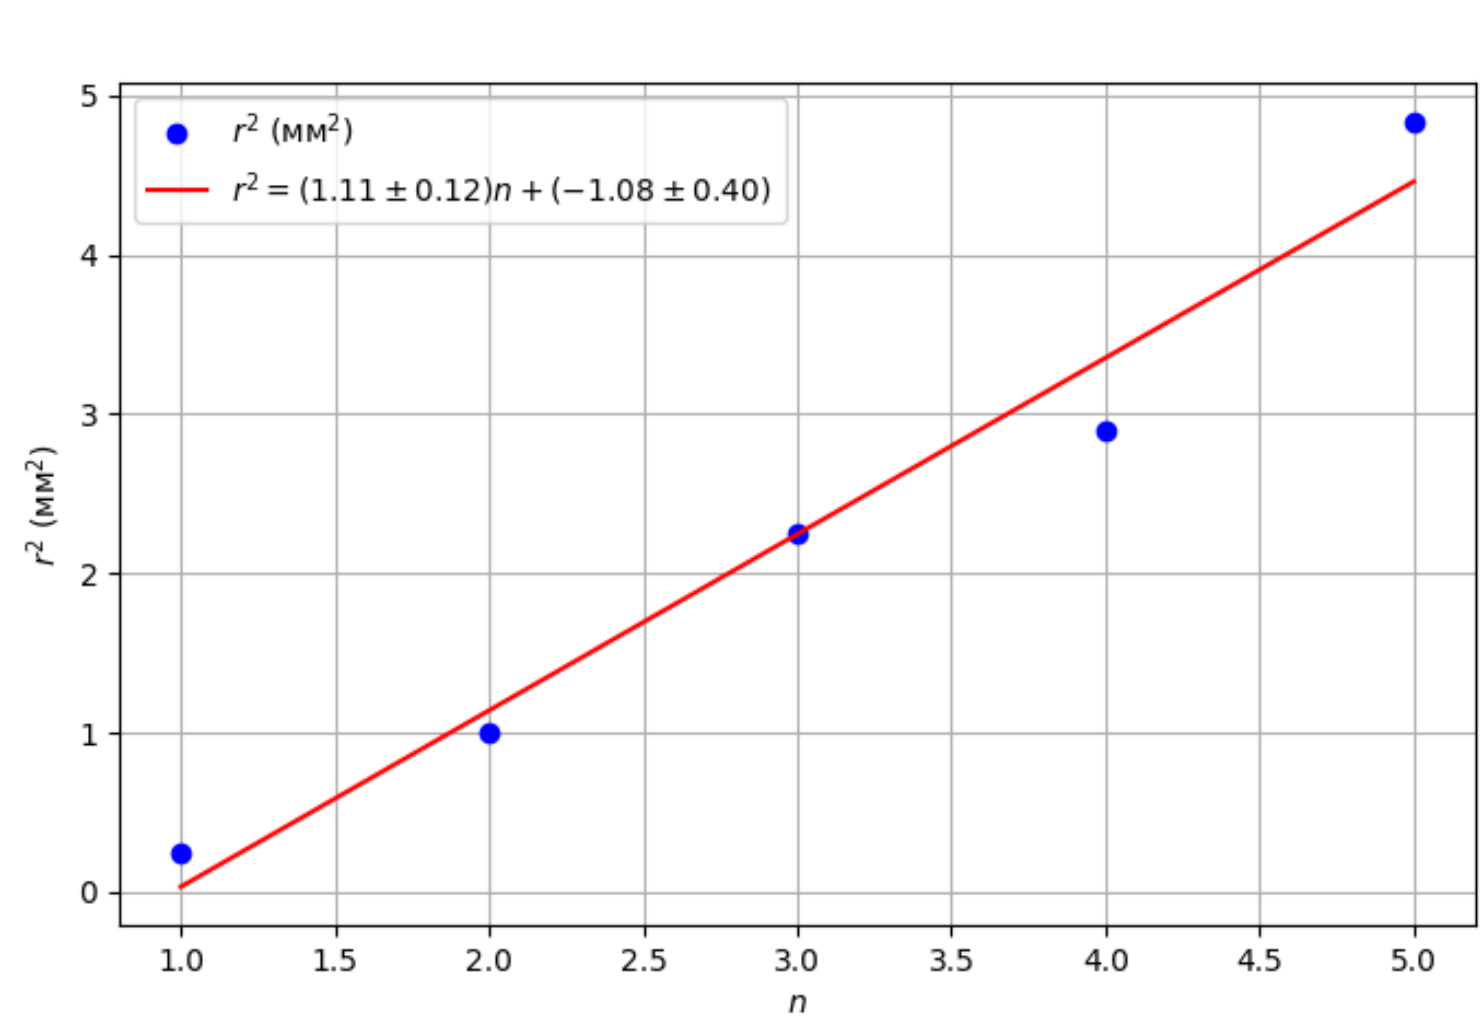
\includegraphics[width=0.9\linewidth]{figures/r^2(n).png}
		      \caption{Зависимость $r^2$ от $n$}
	      \end{figure}
	      \\
	      Теорическое значение:
	      \[
		      \frac{\D r_n^2}{\D n} = \frac{2 L (L - a)}{m_0} = (1.11 \pm 0.12) \mm^2
	      \]
	      Реальное значение:
	      \[
		      \frac{2 L (L - a)}{m_0} = 1.2 \mm^2
	      \]

	\item Измерим ширину полос. \\
	      Получим вертикальные полосы. \\
	      Сместим центр и.к. от центра экрана (т. $O^'$). \\
	      Измерим шируну центральной полосы и $OO^'$.
	      \[
		      OO^{'} \approx 3 \mm
	      \]
	      \[
		      \theta = \frac{1}{2} \frac{OO^{'}}{L} \approx 0.1\dg
	      \]
\end{enumerate}

\section{Измерение длины волны лазерного излучения}
Включим частотометр и осциллограф. \\
Включим двигатель. \\
Запишем результаты подсчета для нескольких циклов работы двигателя. \\
\begin{table}[H]
	\centering
	\begin{tabular}{|l|l|l|l|l|l|l|l|}
		\hline
		$n$       & 1   & 2   & 3   & 4   & 5   & 6   & 7   \\
		\hline
		$N, 10^3$ & 144 & 126 & 132 & 121 & 127 & 124 & 129 \\
		\hline
	\end{tabular}
\end{table}

При выполнении, у нас получались большие выбросы. N принимало значения от 100 до 500. \\
В таблице записаны наиболее согласованные с теорией значения. \\
В народе такой метод называют ``подгон``.

\begin{gather*}
	\avrg{N} = 129 \pm 8\\
	l = 32 \mm \\
\end{gather*}
\begin{gather}
	\text{Формула (2.70)}: \quad
	\lambda = \frac{2l}{N} \\
	\D \lambda = \frac{2l}{N^2} \D N
\end{gather}
\\
Теоретическое значение:
\[
	\lambda = 6328 \stackrel{\circ}{\mathrm{A}}
\]
Полученное значение:
\[
	\lambda = ( 5000 \pm 30 ) \stackrel{\circ}{\mathrm{A}}
\]

\section{Исследование эффекта Доплера}
Определим частоту колебаний. \\
\begin{equation}
	\nu = \frac{N}{T}
\end{equation}
$T$ - период работы двигателя. \\

\begin{equation}
	v = \frac{l}{T}
\end{equation}

\begin{table}[H]
	\centering
	\begin{tabular}{|l|l|l|}
		\hline
		n & $T_n, \sec$ & $v_n, \frac{\mm}{\sec}$ \\
		\hline
		1 & 42 \pm 0.3  & 0.760 \pm 0.004         \\
		\hline
		2 & 82 \pm 0.3  & 0.390 \pm 0.001         \\
		\hline
		3 & 225 \pm 0.3 & 0.1400 \pm 0.0002       \\
		\hline
	\end{tabular}
\end{table}

\begin{table}[H]
	\centering
	\begin{tabular}{|l|l|l|l|}
		\hline
		                  & 1   & 2   & 3   \\
		\hline
		$\nu_1, \kilo\Hz$ & 2.5 & 2.3 & 2.1 \\
		\hline
		$\nu_2, \kilo\Hz$ & 1.7 & 1.5 & 1.6 \\
		\hline
		$\nu_2, \kilo\Hz$ & 1.6 & 1.5 & 1.7 \\
		\hline
	\end{tabular}
\end{table}

\begin{gather}
	\nu_n = \nu_0 \left( 1 - \frac{2 v_n}{c} \right) \\
	\nu_0 = \frac{c}{\lambda} \\
	\D \nu_n = \nu_n - \nu_0 = \frac{2 v_n}{\lambda}
\end{gather}

\begin{figure}[H]
	\centering
	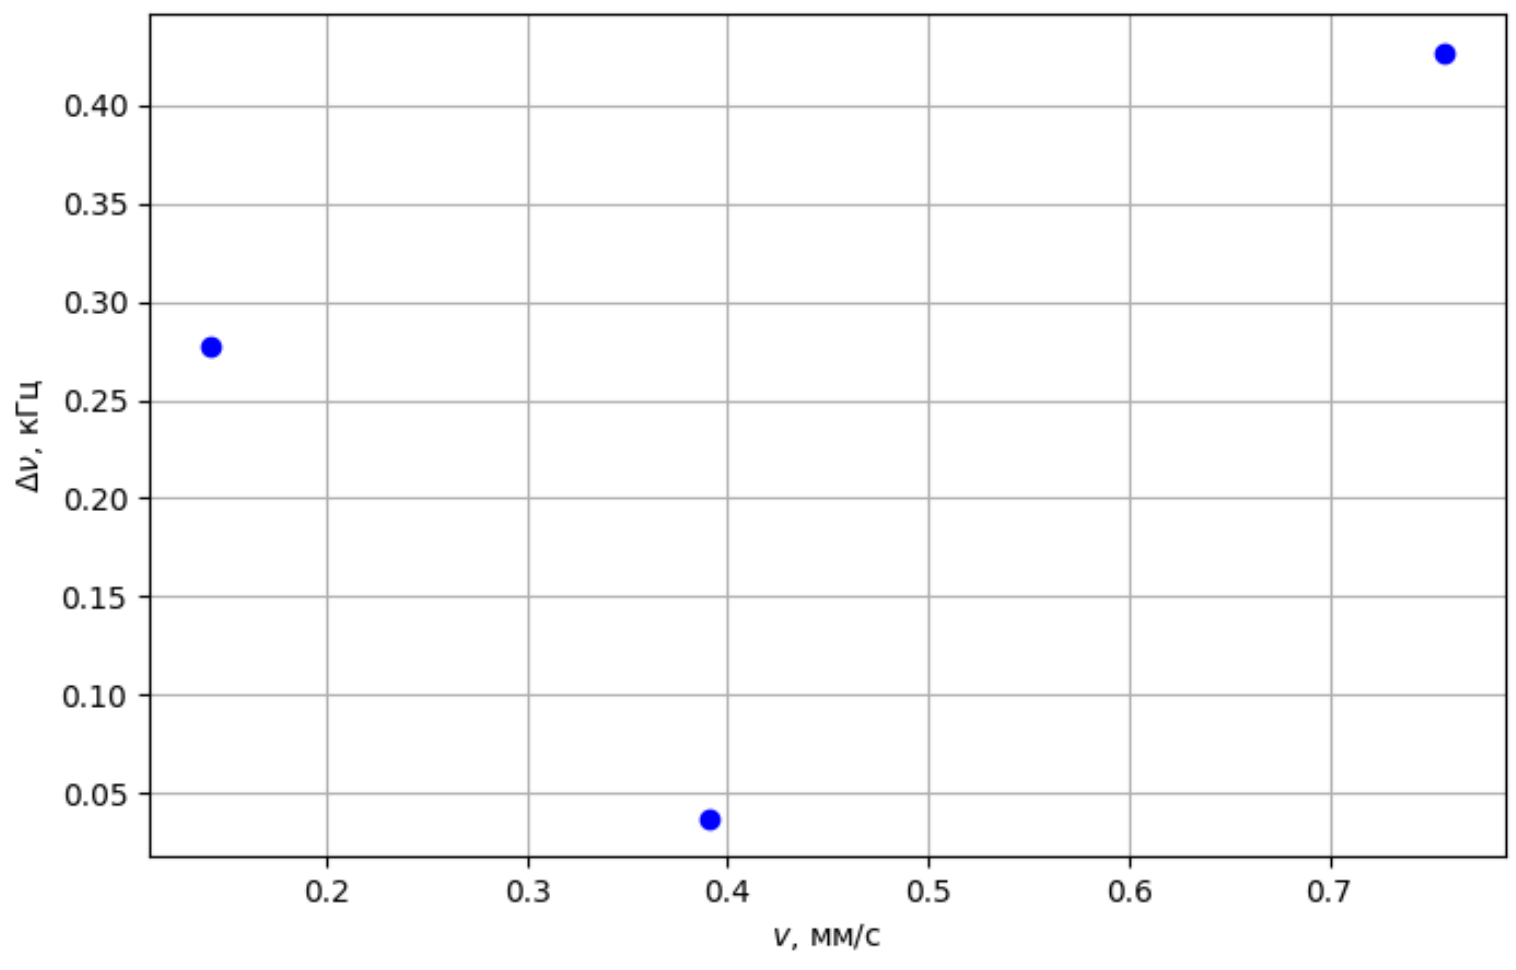
\includegraphics[width=0.9\linewidth]{figures/nu(v).png}
	\caption{Зависимость $\nu$ от $v$}
\end{figure}

\section{Выводы}
В ходе работы мы провели несколько экспериментов с интерферометром Майкельсона.
\begin{enumerate}
	\item Наблюдали интерференционные картины, измерили радиусы тёмных колец.
	      Подтвердили линейную зависимост $r_n^2 \sim n$.

	\item Определили длину волны лазерного излучения по числу проходящих
	      полос, но, видимо, из-за неудачной юстировки результат
	      отклонился от действительного.

	\item Зафиксировали изменение частоты сигнала ФЭУ при движении зеркала.
	      Однако расхождения между сериями систематические.

	\item Построили график зависимости $\D \nu$ от $v$, получили расхождение с
	      теорией, что говорит об отсутствии эффекта Доплера в интерферометре
	      Майкельсона (или о кривоте наших рук).
\end{enumerate}

\end{document}
